\chapter{Experimental Evaluation and Results}  %Title of the First Chapter

\ifpdf
    \graphicspath{{Chapter4/Figs/Raster/}{Chapter4/Figs/PDF/}{Chapter4/Figs/}}
\else
    \graphicspath{{Chapter4/Figs/Vector/}{Chapter4/Figs/}}
\fi

In this chapter we present the quantitatve and qualitative evaluations of our learning algortighms as described in the last chapter.All the experiments are performed on the green channel of the image as it has the maximum contast between the vessel and background as can be seen in Fig \ref{fig:fundus image}.\\
\begin{figure}
	\begin{subfigure}[b]{0.3\textwidth}
		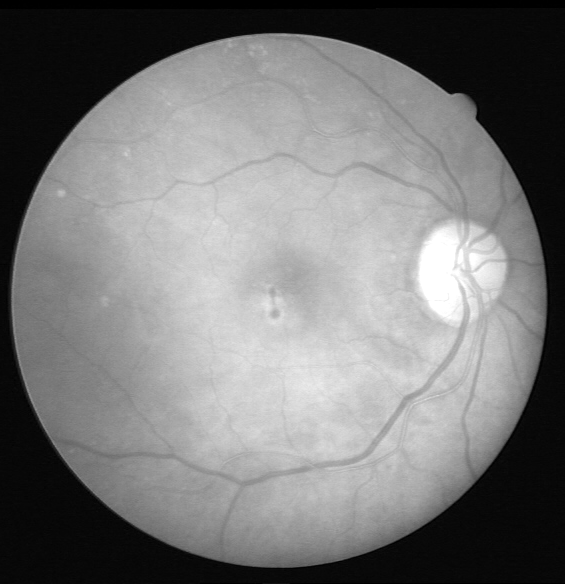
\includegraphics[width=\textwidth]{red.png}
		\caption{Red channel}
		\label{fig:red fundus}
	\end{subfigure}
	%
	\begin{subfigure}[b]{0.3\textwidth}
		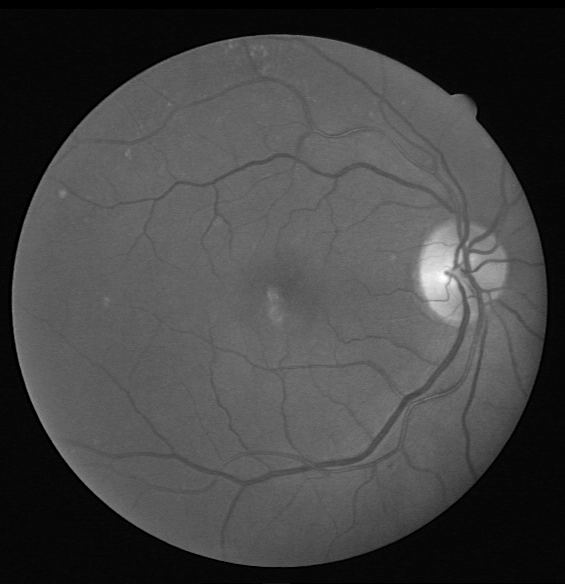
\includegraphics[width=\textwidth]{green.png}
		\caption{Green channel}
		\label{fig:green fundus}
	\end{subfigure}
	\begin{subfigure}[b]{0.3\textwidth}
		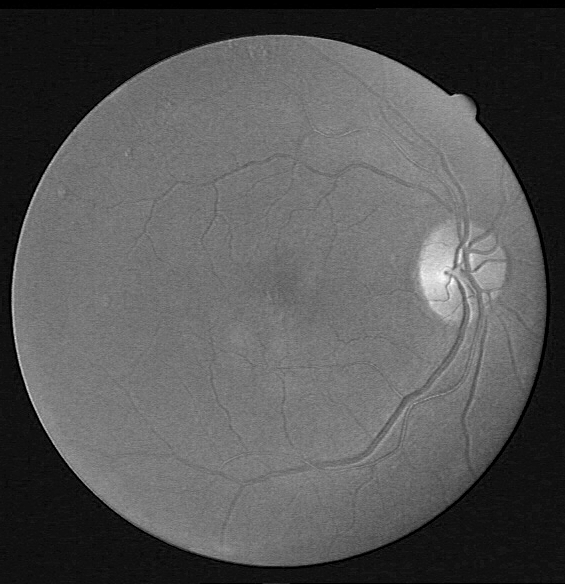
\includegraphics[width=\textwidth]{blue.png}
		\caption{Blue channel}
		\label{fig:blue fundus}
	\end{subfigure}
	\caption[Red, Gree, Blue channels of a fundus image]{Different channels of a fundus image showing variation in contrast of blood vessels against background. Green channel shows the maximum contrast in blood vessels and background.}
	\label{fig:fundus image}
\end{figure}

Ther performance of the proposed vessel segmentation algorithm is evaluated using the segmented vaculature considered as the gold standard and the manually marked segmentations by the human observer.All prior work with which we compare our method, have done a segmentation performance analysis with the manual segmentations provided by the first human observer. Additionally for some of the datasets we have a manual segmentation provided by the second observer which can be used to compare the automated methods to that of manual segmentations.\\

To asses the performance of segmentation methods, various metric have been defined in literature \cite{monteiro2006performance,sharma2001performance}. As reported in prioir works,we also compute the performance of our vessel segmentation model defined as, true positives (TP): number of correctly classified vessel pixels; false positives (FP): number of pixels falsely classified as vessels; true negatives(TN): number of correctly classified non-vessel pixels; false negatives(FN): number of pixels falsely classified as non-vessels.\\

Using these metrics we can compute the accuracy (number of TP+TN / total pixels) ,pixel classification sensitivity and specificity.
We also calculate the area under curve for receiver operation characteristics and also the AUC under the precision recall curve obtained by varying the threshold value for the segmented images.\\

For a complete assesment of our segmentation model, we perform various experiments. We start by performing the experiment on all the 4 datasets and compute the performance metrics as described above. Next, to test the generalization of our system we do cross training, i.e, training on images from one dataset and prediction on other.

We test the performance of both our models.  	

\section{Vessel Segmenetation Assessment}
We start by training our model on the DRIVE training datset. The classifier is trained with a patch size of (10,10) and 1000 clusters. We also run the algorithm with the various preprocessing settings as in sections.Contrast enhancement of the images didn't have a major effect on our performance.\\

We applied our model with varying patch sizes ranging from (10,10) to (21,21). We note that with increase in patch size, we lose details on the thin vessels, but our confidence on thick vessels increases. We combine the results on various patch sizes by simple averaging of all the cases. This had a slight imporvement over our results.

\begin{figure}
	\begin{subfigure}[b]{0.45\textwidth}
		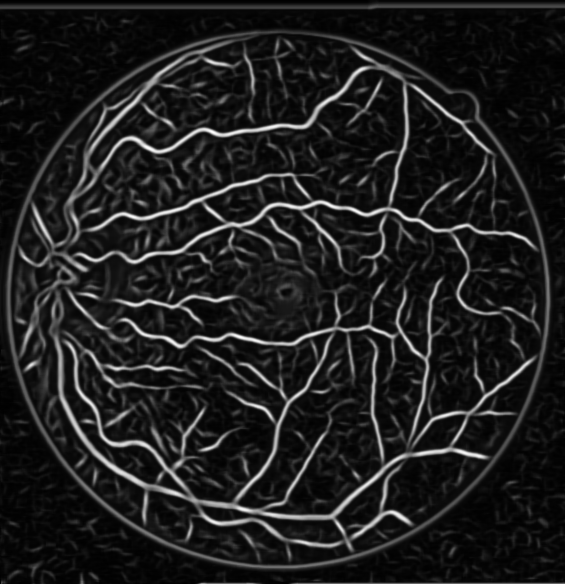
\includegraphics[width=\textwidth]{psize/p10.png}
		\caption{patch size (10,10)}
		\label{fig:p10}
	\end{subfigure}
	%
	\begin{subfigure}[b]{0.45\textwidth}
		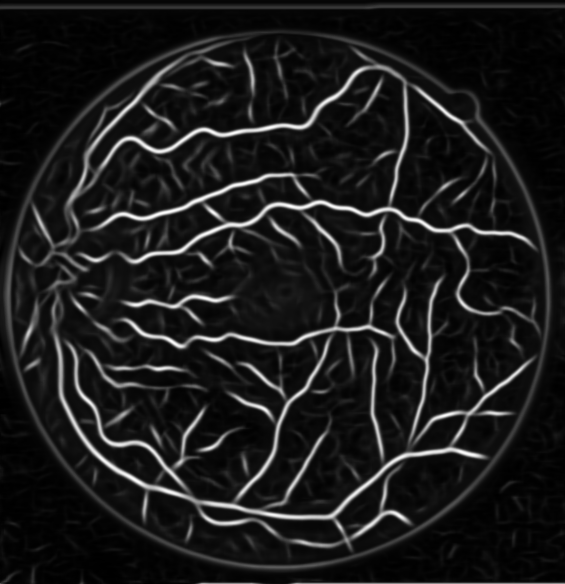
\includegraphics[width=\textwidth]{psize/p15.png}
		\caption{patch size (15,15)}
		\label{fig:p15}
	\end{subfigure}
	
	\begin{subfigure}[b]{0.45\textwidth}
		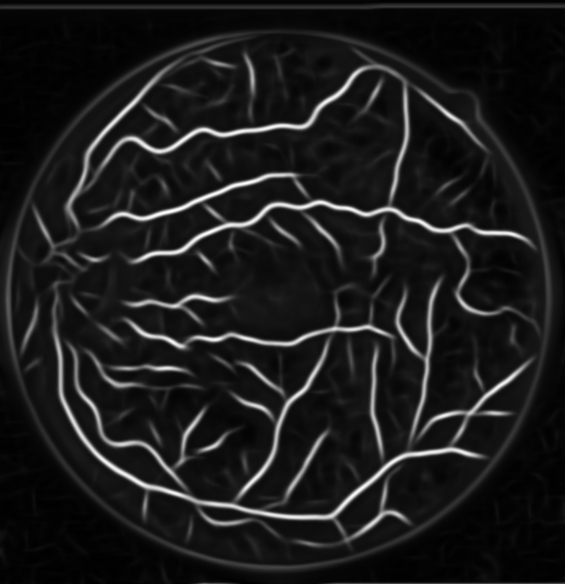
\includegraphics[width=\textwidth]{psize/p21.png}
		\caption{patch size (21,21)}
		\label{fig:p21}
	\end{subfigure}
	\begin{subfigure}[b]{0.45\textwidth}
		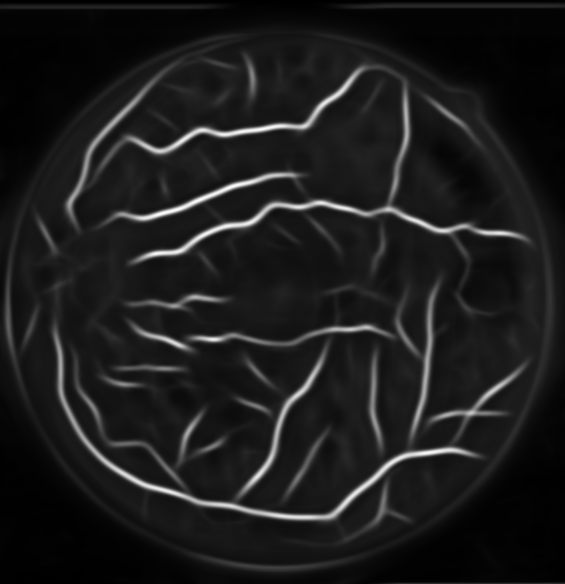
\includegraphics[width=\textwidth]{psize/p33.png}
		\caption{patch size (33,33)}
		\label{fig:33}
	\end{subfigure}
	\caption[Image segmentation using varying patch sizes]{Here we show the effect of varying patch size in our patch based framework. As we increase the patch size, we lose details on thin vessels,but our confidence on thick vessess increases.}
	\label{fig:patch size}
\end{figure}

Results for our model applied on DRIVE test datset are shown in the table. As we obtain an average value at each pixel by merging the ground truth annotation coming from different overlapping patches, we can threshold the intensities to obtain the binar segmentation.ROC and PRC plots are made by varying the thresholds in steps of 0.02.

